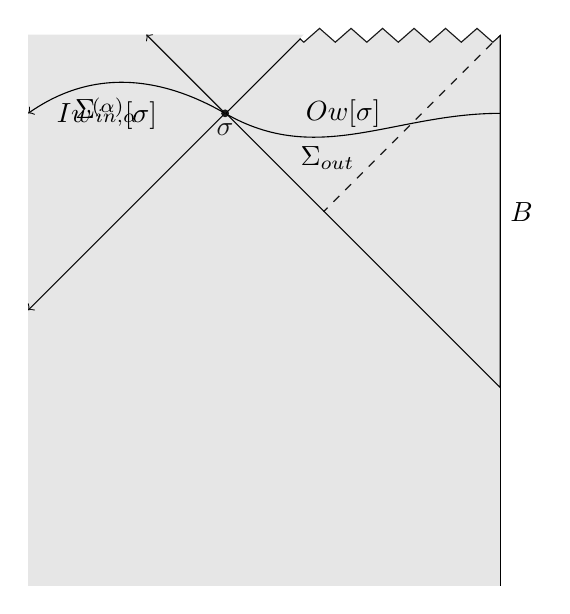
\begin{tikzpicture}

  \coordinate (bl) at (0, 0);
  \coordinate (tl) at (0, 7);
  \coordinate (tr) at (6, 7);
  \coordinate (br) at (6, 0);
  \coordinate (owtl) at (4.5, 8);
  \coordinate (owtr) at (6 ,8);
  \coordinate (iwtr) at (1.5, 7);
  \coordinate (iwtl) at (0, 7);
  \coordinate (iwbl) at (0, 3.5);
  \coordinate (owbr) at (6, 2.5);
  \coordinate (ehb) at (0, 1);
  \coordinate (iwlab) at (1,6);
  \coordinate (owlab) at (4,6);

  \coordinate (sig) at (2.5, 6);
  \coordinate (sigout) at (6, 6);
  \coordinate[label=right:$B$] (asdf) at (6, 4.75);
  \coordinate (sigin) at (0, 6);
  \coordinate (bdry) at (6, 4.75);

  \begin{scope}[decoration={zigzag, segment length=0.4cm}]
    \draw[dashed, opacity=0] (tl) to (bl);
    \draw[dashed, opacity=0] (tr) to (br);

    \node at (sig)[circle,fill,inner sep=1pt]{};
    \coordinate[label=below:$\sigma$] (sig) at (2.5, 6);

    \begin{scope}
      \path[clip] (tl) decorate {to (tr)} to (br) to (bl) -- cycle;
      \path[clip] (sig) to (owtl) to (owtr) to (owbr) -- cycle;

      \draw[decorate, thick] (tr) to (tl);
      \draw[dashed] (ehb) to (tr);

      \draw[fill=gray, fill opacity=0.2, thick] (sig) to (owtl) to (owtr) to (owbr) to (sig);

    \end{scope}

    \onslide<6->{
      \draw[fill=gray, opacity=0, fill opacity=0.2] (sig) to (iwtr) to (iwtl) to (iwbl) to (sig);
      \draw[->] (sig) to (iwtr);
      \draw[->] (sig) to (iwbl);
    }
    \onslide<6>{
      \node at (iwlab) {$Iw^{(\alpha)}[\sigma]$};
    }


    \onslide<-6>{
      \node at (owlab) {$Ow[\sigma]$};
    }

    \onslide<7->{
      \coordinate[label=below:$\Sigma_{out}$] (sigoutlab) at (3.8, 5.7);
      \coordinate[label=below:$\Sigma_{in,\alpha}$] (siginlab) at (1, 6.3);
      \draw[out=-30, in=180] (sig) to (sigout);
      \draw[<-, out=35, in=150] (sigin) to (sig);
    }

    \onslide<8->{
      \draw[fill=gray, opacity=0, fill opacity=0.2] (sig) to (iwbl) to (bl) to (br) to (owbr) -- cycle;
      \draw[fill=gray, opacity=0, fill opacity=0.2] (sig) to (3.5,7) to (1.5,7) -- cycle;
      \draw (tr) to (br);
    }



  \end{scope} 



\end{tikzpicture}
